%%%%%%%%%%%%%%%%%%%%%%%%%%%%%%%%%%%%%%%%%
% Beamer Presentation
% LaTeX Template
% Version 1.0 (10/11/12)
%
% This template has been downloaded from:
% http://www.LaTeXTemplates.com
%
% License:
% CC BY-NC-SA 3.0 (http://creativecommons.org/licenses/by-nc-sa/3.0/)
%
%%%%%%%%%%%%%%%%%%%%%%%%%%%%%%%%%%%%%%%%%

%----------------------------------------------------------------------------------------
%	PACKAGES AND THEMES
%----------------------------------------------------------------------------------------

\documentclass[graphics]{beamer}

\mode<presentation> {

% The Beamer class comes with a number of default slide themes
% which change the colors and layouts of slides. Below this is a list
% of all the themes, uncomment each in turn to see what they look like.

%\usetheme{default}
%\usetheme{AnnArbor}
%\usetheme{Antibes}
%\usetheme{Bergen}
%\usetheme{Berkeley}
%\usetheme{Berlin}
%\usetheme{Boadilla}
%\usetheme{CambridgeUS}
%\usetheme{Copenhagen}
%\usetheme{Darmstadt}
%\usetheme{Dresden}
%\usetheme{Frankfurt}
%\usetheme{Goettingen}
%\usetheme{Hannover}
%\usetheme{Ilmenau}
%\usetheme{JuanLesPins}
%\usetheme{Luebeck}
\usetheme{Madrid}
\usepackage{mathtools,amsmath,amsthm,bm}

%\usetheme{Malmoe}
%\usetheme{Marburg}
%\usetheme{Montpellier}
%\usetheme{PaloAlto}
%\usetheme{Pittsburgh}
%\usetheme{Rochester}
%\usetheme{Singapore}
%\usetheme{Szeged}
%\usetheme{Warsaw}

% As well as themes, the Beamer class has a number of color themes
% for any slide theme. Uncomment each of these in turn to see how it
% changes the colors of your current slide theme.

%\usecolortheme{albatross}
%\usecolortheme{beaver}
%\usecolortheme{beetle}
%\usecolortheme{crane}
%\usecolortheme{dolphin}
%\usecolortheme{dove}
%\usecolortheme{fly}
%\usecolortheme{lily}
%\usecolortheme{orchid}
%\usecolortheme{rose}
%\usecolortheme{seagull}
%\usecolortheme{seahorse}
%\usecolortheme{whale}
%\usecolortheme{wolverine}

%\setbeamertemplate{footline} % To remove the footer line in all slides uncomment this line
%\setbeamertemplate{footline}[page number] % To replace the footer line in all slides with a simple slide count uncomment this line

%\setbeamertemplate{navigation symbols}{} % To remove the navigation symbols from the bottom of all slides uncomment this line
}

\usepackage{color}
\usepackage{graphicx} % Allows including images
\usepackage{booktabs} % Allows the use of \toprule, \midrule and \bottomrule in tables
\usepackage{cancel}
\usepackage[absolute,overlay]{textpos}
%\usepackage{movie15}
%\usepackage{multimedia,lmodern}
%\usepackage{media9}
\graphicspath{ {./figure/}  {/Users/ginochen/Gino/Paper/Paper_QJRMS/paper_final_revision/} {/Users/ginochen/Gino/IEPC/paperplot/figures/epsFig/} }

\newcommand{\overbar}[1]{\mkern 1.5mu\overline{\mkern-1.5mu#1\mkern-1.5mu}\mkern 1.5mu}

%----------------------------------------------------------------------------------------
%	TITLE PAGE
%----------------------------------------------------------------------------------------

\title[Efficient Perturbed Parameter Scheme] {An Efficient Perturbed Parameter Scheme in the Lorenz system for Quantifying Model Uncertainty} % The short title appears at the bottom of every slide, the full title is only on the title page

\author[Gino Chen et al ]{Gino Chen, Ben Kirtman and Mohamed Iskandarani} % Your name
\institute[University of Miami] % Your institution as it will appear on the bottom of every slide, may be shorthand to save space
{ University of Miami\\ % Your institution for the title page
\medskip
\textit{} % Your email address
}
\date{} % Date, can be changed to a custom date

\AtBeginDocument{%
  \setlength\abovedisplayskip{0pt}
  \setlength\belowdisplayskip{0pt}}

\begin{document}

  
\begin{frame}
\titlepage % Print the title page as the first slide
\end{frame}


%\begin{frame}
%\frametitle{Overview} % Table of contents slide, comment this block out to remove it
%\tableofcontents % Throughout your presentation, if you choose to use \section{} and \subsection{} commands, these will automatically be printed on this slide as an overview of your presentation
%\end{frame}

%----------------------------------------------------------------------------------------
%	PRESENTATION SLIDES
%----------------------------------------------------------------------------------------

%%------------------------------------------------
%\section{Introduction} % Sections can be created in order to organize your presentation into discrete blocks, all sections and subsections are automatically printed in the table of contents as an overview of the talk
%%------------------------------------------------
%
%\subsection{Subsection Example} % A subsection can be created just before a set of slides with a common theme to further break down your presentation into chunks

%------------------------------------------------
\begin{frame}[t]
   \frametitle{Motivation}
        % 1) Ignore the boxes, you see the true topography, and a flow that accelerates over the top and bottom but is slowed down in the center where gravity wave drag kicks in.
        % 2) When you have a coarse grid, the gravity wave drag is uniformly parameterized to the boxes with topography, so all three boxes are decelerated.
	% 3) In truth, the red boxes should have no drag with the given flow!! => shouldn't be uniform!
	% 4) Depending on different flow directions, the drag could be applied to 1 & 3 (i.e., a southerly flow then 1 could recieve a drag with 2 & 3 accelerating)
        % 5) the drag should be a constantly varying parameterization!! => stochastic parameterization
      \begin{itemize}
         \item {\bf Models contain serious errors!} % forecast bias!
             \includegraphics[width=0.8\textwidth, height=0.55\textwidth]{drag_param} 
		\flushright{Palmer 2006}
      \end{itemize}
\end{frame}

\begin{frame}[t]
   \frametitle{Motivation}
      \begin{itemize}
         \item  {\bf Bulk-parameterized wave-drag tendency causing error!} % forecast bias!
               \includegraphics[width=0.8\textwidth, height=0.55\textwidth]{drag_param_bulk_turb} 
		%\flushright{Palmer 2006}
      \end{itemize}
\end{frame}

\begin{frame}
   \frametitle{Approach}
	% 1) follow from the previous slide, add a constantly varying term
	% 2) Stop kicking the tendency term constantly? 
        % 3) fixed perturbation throught the model simulation, still reliable? Can we achieve equivalent skill?
        % 4) can we save some cost?
	% 5) Use informative probability distribution of the perturbed parameter in the parameterized tendency, this will be defined later
	% 6) Fourier-like series expansion (PCE) on the uncertainty space
      \begin{itemize}
         \item Add stochastisity to the bulk-parameterized term.  %mimic the subgrid fluctuation 
		\begin{itemize}
		   \item Additive {\bf Stochastic Parameterization } \vspace{30pt}
		\end{itemize}
         \item Without stochastisity in time? Still reliable?
		\begin{itemize}
		   \item Proposed scheme: ``Informative" {\bf Perturbed Parameter} scheme  \\
		   \vspace{12pt}
		   $\Longrightarrow$ Cost reduction with spectral method!
		\end{itemize}
      \end{itemize}
\end{frame}

\begin{frame}
   \frametitle{Experimental Setup}
	\begin{itemize}
	   \item Model equations: Lorenz'63 \& Lorenz'96
		\vspace{12pt}
	   \item Truth model \& Parameterized forecast model
		\vspace{12pt}
	   \item 300 perfect initial conditions 
	\end{itemize}
\end{frame}

\begin{frame}
   \frametitle{Experimental Setup}
	% 1) given a coupled Lorenz 63 system and a Lorenz 96 system (with 4 grid points representing the spatially resolve subgrid processes)
	% 2) the subgrid system Z could be seen as a cloud-scale process couple to the atmosphere.
        % 3) F's are the nonlinear operators, I simplified the model to focus on the important bulk-parameterized tendency term U, here the truth U coupled to the subgrid Z
	% 4) Ocean has a shorter time separation which has slower varying dynamics
	% 5) The entire system of equations gives the true states
	% 6) Perfect initial conditions are used for comparing only model errors.
	\begin{itemize}
           \item {\color{blue} Truth} model
	      \begin{itemize}
	         \item Atmosphere
	            \begin{equation*}
		    \begin{aligned}
	                & \frac{d \vec{X}}{d t} = F_x(\vec{X},\vec{Y}) + {\color{blue} \text{U}_{\text{truth}}(\vec{Z})} \\
                        & \frac{d Z_i}{d t} = F_z(\vec{Z},X); \ \ i=1, \dotsc, 4
                    \end{aligned}
                    \end{equation*}
	         \item Ocean
	            \begin{equation*}
	                \hspace{-70pt} \frac{d \vec{Y}}{d t} = F_y(\vec{X},\vec{Y})
	            \end{equation*}
              \end{itemize}
	\end{itemize}
\end{frame}

\begin{frame}
   \frametitle{Experimental Setup}
	% 1) when truncating the subgrid system Z, U_truth is parameterized by U_p(X), this is when model start to have errors!!
	% 2) The following section will show three schemes to parameterize U_truth
	\begin{itemize}
           \item {\color{red} Parameterized} forecast model
	      \begin{itemize}
	         \item Atmosphere
	            \begin{equation*}
		    \begin{aligned}
	               & \frac{d \vec{X}}{d t} = F_x(\vec{X},\vec{Y}) + {\color{red} \text{U}_{\text{param}}(X)} \\
                       & {\cancel{ \frac{d Z_i}{d t} = F_z(\vec{Z},X) }}; \ \ i=1, \dotsc, 4 
	            \end{aligned}
                    \end{equation*}
	         \item Ocean
	            \begin{equation*}
	               \hspace{-70pt} \frac{d \vec{Y}}{d t} = F_y(\vec{X},\vec{Y})
	            \end{equation*}
                 
              \end{itemize}
	\end{itemize}
\end{frame}


\begin{frame}
	% 1) This figure shows the relationship of U_truth as a function of the atmospheric variable X, this is the state space of U we try to parameterize
	% 2) The time samples of U is the cloud of blue dots. Remember, blue is true U_truth.
   \frametitle{A cloud of $\text{U}_{\text{truth}}$}
   \vspace{20pt}
   {\color{blue}  $\text{U}_{\text{truth}}(X)$ } 
   \includegraphics[width=0.9\textwidth, height=0.55\textwidth]{stoch_cloud_final}
\end{frame}

\begin{frame} % magenta to stoch variable, make a magenta cloud for stoch
	% 1) So the bulk-parameterization is to fit a deterministic curve through the cloud of truth points
	% 2) Thus U time samples are fixed on the red curve
	% 3) At any time instance, we have a pair of truth blue dot and parameterized red dot, the distance between the two is the true error e_truth
	% 4) In order to capture the true error, we add a stochastisity to the deterministic curve, which becomes the e_stoch
	% 5) The e_stoch is modeled with correlation obtained from the true e_truth, we will skip the details and focus on the next scheme, which is our main focus and innovation
   \frametitle{$\text{U}_{\text{param}}$: Deterministic \& Stochastic}
      ${\color{black} \text{U}_{\text{det}} = b_0 + b_1X + b_2X^2 + b_3X^3}$, \\
      \vspace{8pt}
      ${\color{blue} \text{U}_{\text{truth}}} = {\color{black} \text{U}_{\text{det}}} + {\color{blue} e_{\text{truth}}}$
      \includegraphics[width=0.9\textwidth, height=0.55\textwidth]{stoch_cloud_finalcurve_black}
\end{frame}

\begin{frame}
   \frametitle{$\text{U}_{\text{param}}$: Deterministic \& Stochastic}
      ${\color{black} \text{U}_{\text{det}} = b_0 + b_1X + b_2X^2 + b_3X^3}$, \\
      \vspace{8pt}
      ${\color{blue} \text{U}_{\text{truth}}} = {\color{black} \text{U}_{\text{det}}} + {\color{blue} e_{\text{truth}}}$ $\Longrightarrow$
      ${\color{magenta} \text{U}_{\text{stoch}}} = {\color{black} \text{U}_{\text{det}}} + {\color{magenta} e_{\text{stoch}}}$.
      \includegraphics[width=0.9\textwidth, height=0.55\textwidth]{stoch_cloud_finalcurve_stochparam}
\end{frame}

\begin{frame}% add a pdf for the black curve
	% 1) Instead of using a time-varying parameter e to capture the e_truth, we use a time-fixed constant perturbation e_pert throughout each model realization
	% 2) For instance, at e_pert=0.4, the model uses the black curve, which is just a constant shift from the U_det
	% 3) But we cannot just sample arbitrarily according to these black lines
	% 4) Our study focuses on building a cost effective scheme, which is achieved by perturbed parameter scheme
   \frametitle{$\text{U}_{\text{param}}$: Perturbed Parameter} 
   \vspace{20pt}
  % $  \text{U}_{\text{pert}} = {\color{red} \text{U}_{\text{det}}} + e_{\text{pert}} $. \\
   $  {\color{red} \text{U}_{\text{pert}} } = {\color{black} \text{U}_{\text{det}}} + {\color{red} e_{\text{pert}} } $. \\
   \includegraphics[width=0.9\textwidth, height=0.55\textwidth]{stoch_cloud_finalcurve_pert_single} 
\end{frame}

\begin{frame}
   \frametitle{$\text{U}_{\text{param}}$: Perturbed Parameter} 
   \vspace{20pt}
   $  {\color{red} \text{U}_{\text{pert}} } = {\color{black} \text{U}_{\text{det}}} + {\color{red} e_{\text{pert}} } $. \\
   \includegraphics[width=0.9\textwidth, height=0.55\textwidth]{stoch_cloud_finalcurve_pert_swath} 
\end{frame}

\begin{frame}
	% 0) The lhs pdf is from all the e_truth in the rhs figure
	% 1) We propose to sample e_pert using the e_truth samples. i.e., more samples in the center and less in the outskirts.
	% 2) this lhs pdf is defined as the "informative" distribution.
	% 3) what if we want to use large numbers of perturbed parameter e_pert to reach statistical consistency, but keeping at a low cost? => next section PCE
   \frametitle{Informative Distribution}
   \vspace{37pt}
%   $  {\color{red} \text{U}_{\text{pert}} } = {\color{black} \text{U}_{\text{det}}} + {\color{red} e_{\text{pert}} } $. \\
       \includegraphics[width=0.5\textwidth, height=.55\textwidth]{hist_r_exp1_truth_black} % these are the points to obtain the spectral coefficients for a smooth approximation of the states
   \includegraphics[width=0.5\textwidth, height=.55\textwidth]{stoch_cloud_finalcurve} % these are the points to obtain the spectral coefficients for a smooth approximation of the states
\end{frame}

\begin{frame}
   \frametitle{Informative Distribution}
   \vspace{20pt}
   $  {\color{red} \text{U}_{\text{pert}} } = {\color{black} \text{U}_{\text{det}}} + {\color{red} e_{\text{pert}} } $. \\
       \includegraphics[width=0.5\textwidth, height=.55\textwidth]{hist_r_exp1_pert_black} % these are the points to obtain the spectral coefficients for a smooth approximation of the states
   \includegraphics[width=0.5\textwidth, height=.55\textwidth]{stoch_cloud_finalcurve_pert_swath} % these are the points to obtain the spectral coefficients for a smooth approximation of the states
\end{frame}

\begin{frame} %change the f to x related to X
	% Polynomial Chaos Expansion (PCE)
	% 0) Build a surrogate model, socalled (Polynomial Chaos Expansion (PCE)) %is a function of $e_s$ which could be expanded as a spectral series of the form
	% 1) converge spectrally fast to the exact state
	% 2) use minimal points (quadrature points) to build
	% 3) allows statistics to converge at large ensemble 
	% 4) Once the surrogate is built, plug in the informative distribution and get a ensemble forecast state outputs.
   \frametitle{Cost Reduction}% by spectral methods}
   Fourier-like expansion of the atmospheric and oceanic {\bf state variables}
   \begin{equation*}
      X \ \approx \ x(t,{\color{red} e_{\text{pert}}}) = \sum\limits_{i=1}^N x_i(t) P_i({\color{red} e_{\text{pert}}})
   \end{equation*}
   \includegraphics[width=0.9\textwidth, height=0.45\textwidth]{pce} 
\end{frame}

\begin{frame}
   \frametitle{Summary of the Proposed Scheme}%Efficient Perturbed Parameter Scheme}
	\begin{itemize}
	   \item Build the {\bf surrogate model} for the forecast state variables. % obtain PC coeffients from quadrature rule (psuedospectral projection), do something like a inverse Fourier transform to build the expansion
		\vspace{12pt}
	   \item {\bf Sample the ``input"} ${\color{red} e_{\text{pert}}}$ with an {\bf informative distribution}.
		\vspace{12pt}
	   \item {\bf Obtain the ``output"} ensemble forecast states.
	\end{itemize}
\end{frame}

\begin{frame}
   \frametitle{Forecast Skill}
	% 0) Three standard scores to verify forecast skill: RPSS, IGNSS, REL. I will skip the definition of the skill scores and focus on how well the proposed scheme does
	% 1) left panels represent atmospheric state forecast skill scores as a function of forecast lead times.
	% 2) Det param ill-preformed in all score, which is expected, since it does not capture the subgrid-scale fluctuation. So we focus on the two schemes pert and stoch
	% 3) we want higher scores for the top two scores RPSS and IGNSS, as shown pert gives consistent results
	% 4) REL the lower means more reliable, which is better, and as shown pert also performed well.
	% 5) notice the scores of stoch did not perform well where the reason may be due to the selection of a Gaussion noise in the random walk which is discussed in the paper.
   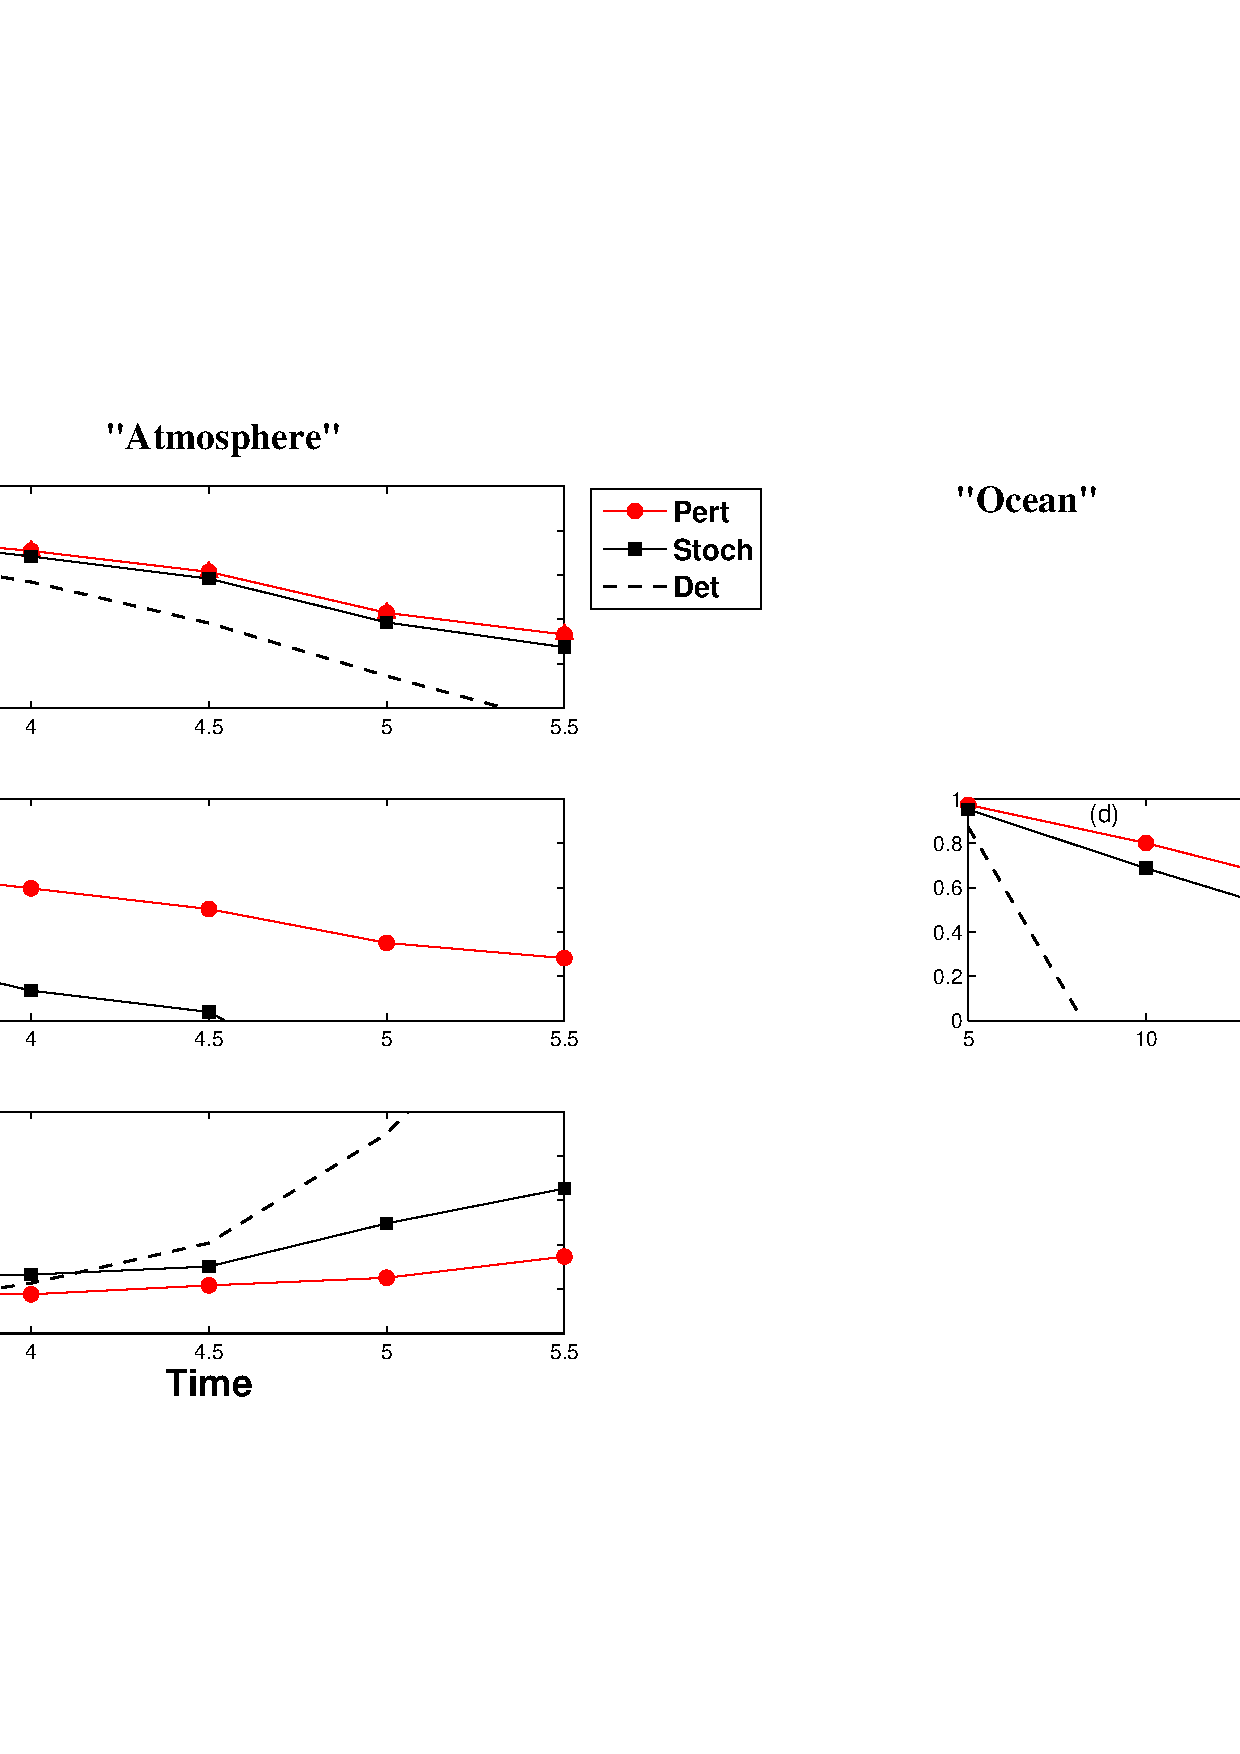
\includegraphics[width=0.5\textwidth, height=0.65\textwidth]{timeseries_eclim_stoch_det_std00_lev8_40pt_meanao_exp1_atm.png}
\end{frame}

\begin{frame}% pert change to black, and others to grey
   \frametitle{Forecast Skill}
   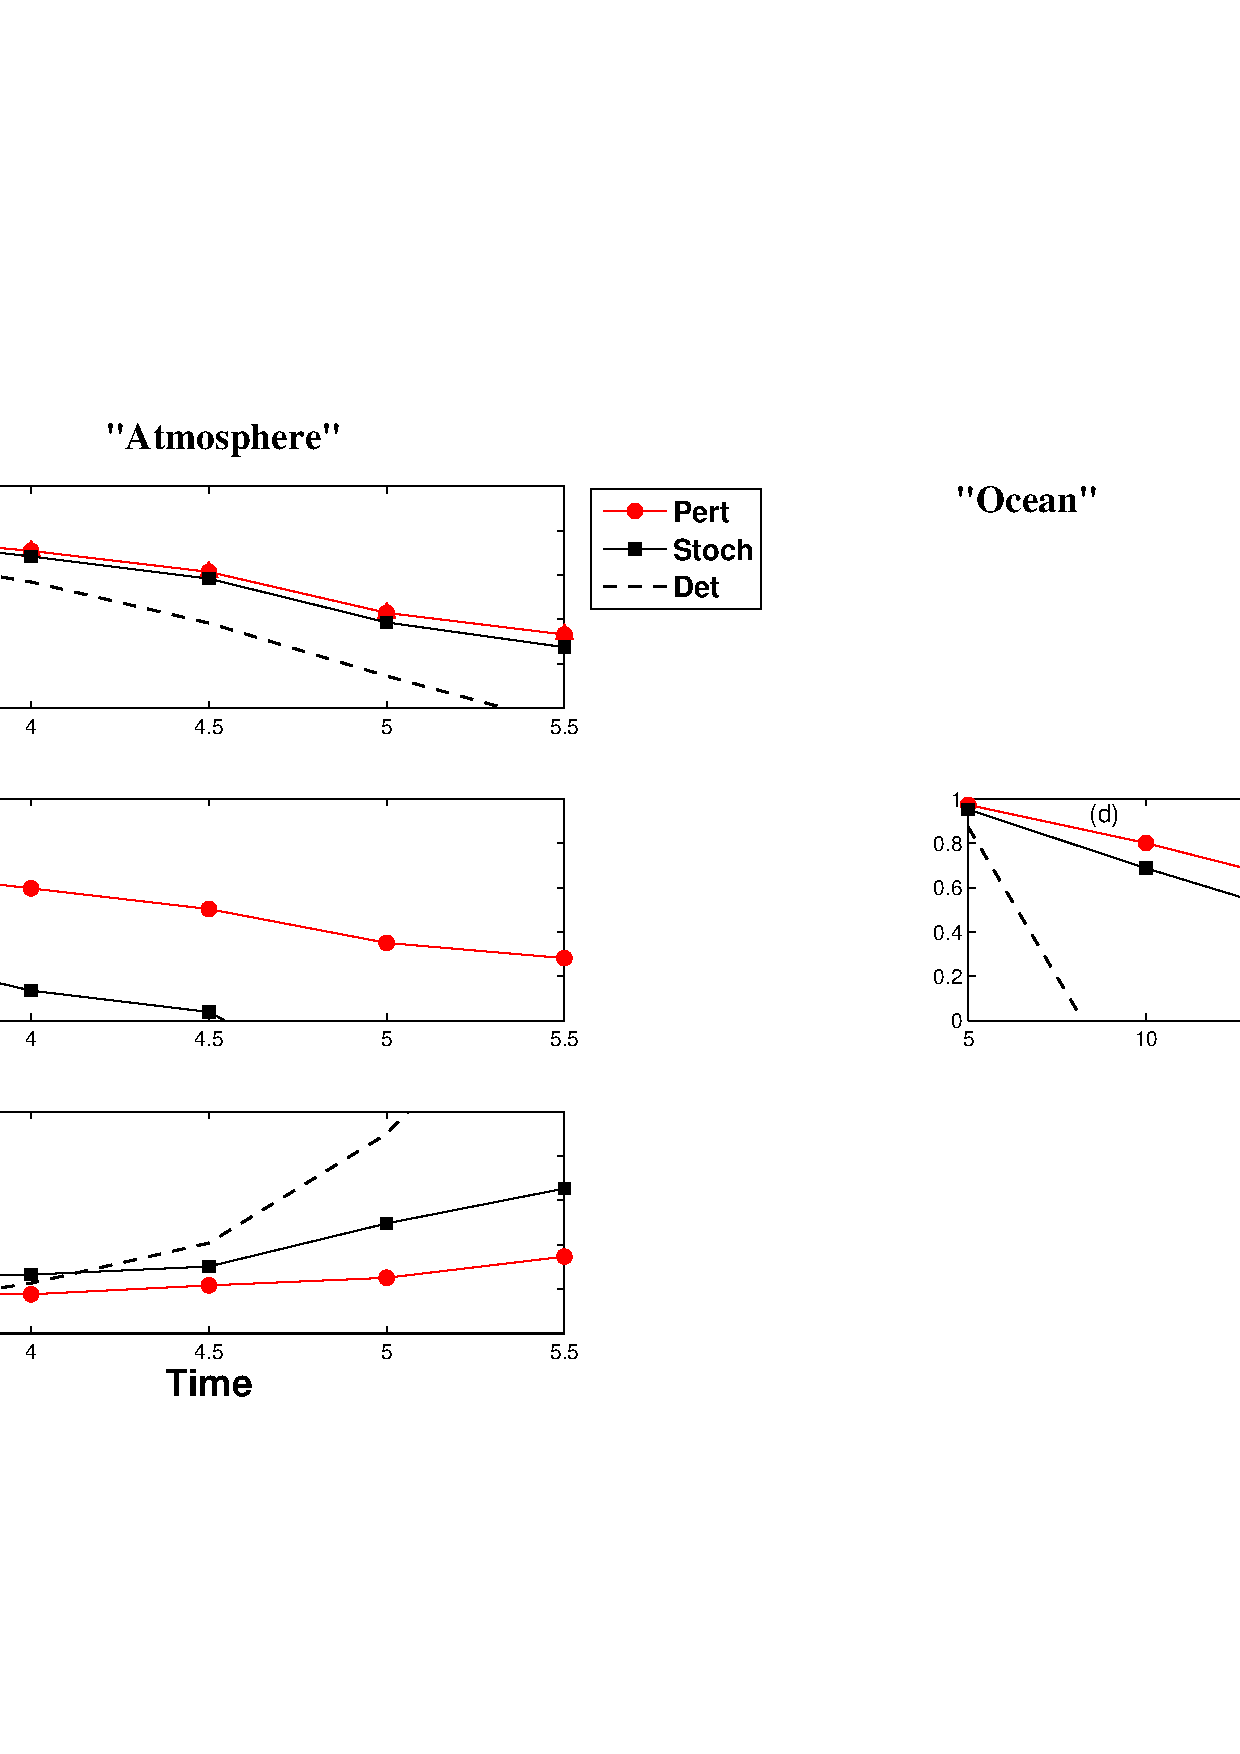
\includegraphics[width=0.5\textwidth, height=0.65\textwidth]{timeseries_eclim_stoch_det_std00_lev8_40pt_meanao_exp1_atm.png}
   \includegraphics[width=0.5\textwidth, height=0.65\textwidth]{timeseries_eclim_stoch_det_std00_lev8_40pt_meanao_exp1_ocn.png}
\end{frame}

\begin{frame}
   \frametitle{Conclusion}
	\begin{itemize}
           \item {Perturbed Parameter Scheme} is {\bf reliable} with ``\emph{informative}" distribution! \\
		\vspace{12pt}
	   \item Polynomial Chaos Expansion further {\bf reduces the cost}. \\ % by converging spectrally fast to the exact solution.
		\vspace{12pt}
	   \item {\bf Easy to apply} to complex GCMs.
	\end{itemize}
\end{frame}

\begin{frame}
   \frametitle{Reference}
	\begin{itemize}
	   \item G Chen, BP Kirtman, and M Iskandarani, \emph{An Efficient Perturbed Parameter Scheme in the Lorenz system for Quantifying Model Uncertainty.} Q. J. Roy. Meteor. Soc. (submitted)
		\vspace{12pt}
	   \item Arnold HM, Moroz IM and Palmer TN. 2013, \emph{Stochastic Parametrizations and Model Uncertainty in the Lorenz'96 System.}, Philos. Trans. A Math. Phys. Eng. Sci., 371
		\vspace{12pt}
	   \item TN Palmer, \emph{Predictability of weather and climate.} Cambridge University Press, 2006

	\end{itemize}
\end{frame}
\end{document} 
